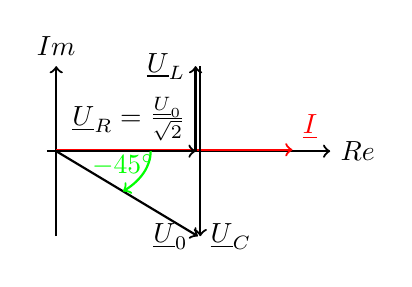
\begin{tikzpicture}[scale=0.6, yscale=0.6, thick]
	%Koordinatensystem
	\draw[->] (-0.2,0) -- +(right:6) node[right] {$Re$};
	\draw[->] (0,-3) -- +(north:6) node[above] {$Im$};
	
	%Pfeile
	\draw[->, color=red] (0,0.05) -- +(right:5) node[above right]
	{$\underline{I}$};
	\draw[->] (0,0) -- +(right:2.95) node[above left] {$\underline{U}_R
	= \frac{\underline{U}_0}{\sqrt{2}}$};
	\draw[->] (2.95,0) -- (2.95,3) node[left]
	{$\underline{U}_L$};
	\draw[->]	(3.05,3) -- (3.05,-3) node[right] {$\underline{U}_C$};
	\draw[->] (0,0) -- (3,-3) node[left] {$\underline{U}_0$};
	
	%Winkel
	\draw[->, color = green] (2,0) arc (0:-45:2) node[above = 2]
	{$-45^{\circ}$};

\end{tikzpicture}


